\documentclass[letterpaper]{article}
%--------------------------------------------------------------------------------
% Useful packages
\usepackage{amsmath}
\usepackage{graphicx,xcolor}
\usepackage{fontspec}
\usepackage[T1]{fontenc}
\usepackage{fancyhdr}
\usepackage{comment}
\usepackage{float}
\usepackage[hidelinks]{hyperref}
\usepackage{xspace}
\usepackage{xurl}
\usepackage{natbib} % the text after reference
\usepackage{microtype}
 \usepackage[strict]{changepage}
 
\setlength{\bibsep}{.5em plus .5em}
\renewcommand{\UrlFont}{\mainfont\fontsize{8.5pt}{8.5pt}\selectfont}

% page setup
\usepackage[letterpaper,top=1.75cm,bottom=1.75cm,left=1.75cm,right=1.75cm, footskip=.75cm]{geometry}
% package ends
%--------------------------------------------------------------------------------




%--------------------------------------------------------------------------------
% font
\newcommand*{\fontdir}[1][font/]{\def\@fontdir{#1}}
\fontdir

% mainbody font
\newfontfamily\mainfont[
  Path=\@fontdir,
  Extension = .ttf,
  UprightFont= *-Regular, % you can also try "*-Light"
  ItalicFont= *-Italic,
  BoldFont= *-Bold,
  BoldSlantedFont = *-BoldItalic,
  FontFace = {l}{n}{*-Light},
   FontFace = {l}{it}{*-LightItalic},
  FontFace = {m}{n}{*-Medium},
%  FontFace = {l}{it}{*-LightItalic},
  FontFace = {sb}{n}{*-Medium},
  FontFace = {sb}{it}{*-MediumItalic},
%  FontFace = {eb}{n}{*-Black},
%  FontFace = {eb}{it}{*-BlackItalic},
]{Roboto}%[LetterSpace=-.25]%, WordSpace=1.25

\DeclareRobustCommand{\smseries}{\fontseries{sb}\selectfont}
\DeclareRobustCommand{\ltseries}{\fontseries{l}\selectfont}
\DeclareRobustCommand{\mdseries}{\fontseries{m}\selectfont}
\DeclareTextFontCommand{\textsm}{\smseries}
\DeclareTextFontCommand{\textmd}{\mdseries}
\DeclareTextFontCommand{\textmi}{\smseries\itshape}
\DeclareTextFontCommand{\textli}{\ltseries\itshape}

\newfontfamily\namefont[
  Path=\@fontdir,
  Extension = .ttf
]{Helvetica-Bold}[LetterSpace=.25]

% head font
\newfontfamily\hfont[
  Path=\@fontdir,
  Extension = .ttf,
  UprightFont= *-Regular,
  ItalicFont= *-Oblique,
  BoldFont= *-Bold,
  SlantedFont= *-Regular
]{Helvetica}


% font ends
%--------------------------------------------------------------------------------



%--------------------------------------------------------------------------------
% color 
% **** change these **** 
\definecolor{gray}{HTML}{888888}
\definecolor{darkgray}{HTML}{222222}
\definecolor{lightgray}{HTML}{aaaaaa} 
\definecolor{verylightgray}{HTML}{efefef} 
\definecolor{mysecondcolor}{HTML}{777777} 
\definecolor{headercolor}{HTML}{3a84cf}
\definecolor{sectioncolor}{HTML}{6196c7}
\definecolor{awardcolor}{HTML}{f5586a}
\definecolor{hookcolor}{HTML}{3a84cf}
% **** **** **** **** **** 
% color ends
%--------------------------------------------------------------------------------




%--------------------------------------------------------------------------------
% section format
\newcommand*{\headregularbigger}[1]{{\hfont\fontsize{16pt}{16pt}\selectfont#1}\space}
\newcommand*{\headregular}[1]{{\hfont\fontsize{16pt}{16pt}\selectfont#1}\space}

\newcommand*{\headboldbigger}[1]{{\hfont\bfseries\fontsize{16pt}{16pt}\selectfont#1}\space}
\newcommand*{\headbold}[1]{{\hfont\bfseries\fontsize{16pt}{16pt}\selectfont#1}\space}
\newcommand*{\headname}[1]{{\namefont\bfseries\fontsize{17pt}{17pt}\selectfont#1}\space}

\newcommand*{\footstyle}[1]{{\mainfont\fontsize{7pt}{7pt}\selectfont\color{mysecondcolor}{#1}}}
\newcommand*{\footstylesmaller}[1]{{\mainfont\fontsize{6.5pt}{6.5pt}\selectfont\color{mysecondcolor}{#1}}}


% section
\usepackage{titlesec} % Used to customize the \section command
\titleformat{\section}{\hfont\bfseries\fontsize{11.5pt}{11.5pt}\selectfont\raggedright}{}{0em}{} % Text formatting of sections
\titlespacing{\section}{1pt}{1pt}{1pt} % Spacing around sections

\titleformat{\subsection}{\hfont\slshape\fontsize{10pt}{10pt}\selectfont\raggedright}{}{0em}{} % Text formatting of sections
\titlespacing{\subsection}{0pt}{0pt}{0pt} % Spacing around sections


\titleformat{\subsubsection}{\hfont\slshape\fontsize{10.5pt}{10.5pt}\selectfont\raggedright}{}{0em}{} % Text formatting of sections
\titlespacing{\subsubsection}{3pt}{0pt}{0pt} % Spacing around sections


\titleformat{\paragraph}[runin]{\smseries\fontsize{9pt}{9pt}\selectfont\raggedright}{\llap{\parbox{\titleindent}{\N\hfill}}}{0em}{}
\titlespacing*{\paragraph}{0pt}{0em plus 0em minus 0em}{.5em plus 0ex}
%--------------------------------------------------------------------------------




%--------------------------------------------------------------------------------
% header 

% Set offset to each header and footer
\fancyhfoffset{0em}
% Remove head rule
\renewcommand{\headrulewidth}{0pt}
% Clear all header & footer fields
\fancyhf{}
% Enable if you want to make header or footer using fancyhdr
\pagestyle{fancy}
\newcommand{\dateseparator}{\raisebox{0pt}{\hspace{2.5pt}{\fontsize{6.5}{6.5}\selectfont{/}}\hspace{2pt}}} %dotsep
\newcommand*{\makefooter}[3]{%
  \fancyfoot[L]{\footstyle{#1} \color{mysecondcolor}{\rule[-1pt]{.5pt}{6pt}} \footstyle{#2}}
  \fancyfoot[C]{}
  \fancyfoot[R]{\footstylesmaller{#3}}
}

% the actually header
\newcommand*{\makeheader}[3]{%
\begin{minipage}{\textwidth}
   \flushleft
	\headname{\color{headercolor}{#1}} \hspace{1pt} \rule[-1.5pt]{1.5pt}{13pt} \hspace{3pt} \headbold{#2}\headregular{#3}
\end{minipage}\vspace*{10pt}%
}


\usepackage{everypage}
\usepackage{tikz}
\AddEverypageHook{  
\begin{tikzpicture}[remember picture,overlay]
\fill[hookcolor,xshift=-30mm,yshift=-248.75mm](0,0) rectangle(7mm,5mm);
\end{tikzpicture}
}

% header ends
%--------------------------------------------------------------------------------

%--------------------------------------------------------------------------------
% last page
\usepackage{lastpage}
% \usepackage{zref-lastpage}
% last page ends
%--------------------------------------------------------------------------------




%--------------------------------------------------------------------------------
%--------------------------------------------------------------------------------
% paragraph
\parindent 0pt
\linespread{1.5} 
\setlength{\parskip}{4pt}
\newcommand{\topicsep}{\vspace{3pt}}
% paragraph ends
%--------------------------------------------------------------------------------



%--------------------------------------------------------------------------------
% reusable notes
%\newcommand{\separator}{\raisebox{0pt}{\hspace{2.5pt}\bfseries{/}\hspace{2pt}}}
% \newcommand*{\separator}{\raisebox{1pt}{\hspace{5pt}\fontsize{3}{3}\selectfont$\bullet$}\hspace{4.5pt}} %\rule{.7pt}{7pt}

\newcommand*{\separator}{\raisebox{0pt}{\hspace{2.5pt}{\fontsize{7}{7}\selectfont{/}}\hspace{2pt}}} %dotsep
\newcommand{\thirdfont}[1]{\fontsize{8}{8}\textli{#1}}
\newcommand{\honorable}{\textsm{\textcolor{awardcolor}{Best Paper Honorable Mention Award}}}
\newcommand{\bestpaper}{\textsm{\textcolor{awardcolor}{Best Paper Award}}}
\newcommand{\honorableOne}{\textsm{\fontsize{9}{9}\selectfont\textcolor{awardcolor}{Best Paper Honorable Mention Award (top 1\%)}}}
\newcommand{\honorableFive}{\textsm{\fontsize{9}{9}\selectfont\textcolor{awardcolor}{Best Paper Honorable Mention Award  (top 5\%)}}}
\newcommand{\bestpaperOne}{\textsm{\fontsize{9}{9}\selectfont\textcolor{awardcolor}{Best Paper Award  (top 1\%)}}}


\newcommand{\etal}{\mbox{et~al.}\xspace}
\newcommand{\ie}{\mbox{i.e.,}\space}
\newcommand{\eg}{\mbox{e.g.,}\space}
\newcommand{\vs}{\mbox{vs.}\space}
\newcommand{\cf}{\mbox{cf.}\space}
\newcommand{\etals}{\mbox{et~al.'s}\space}
\newcommand{\etc}{\mbox{etc.}\space}

%--------------------------------------------------------------------------------




% ------------------------------------------------------------------------------------------------ 
% this is where we disable/enable the notes
% edit tricks
\newif\ifnotes
\notestrue % display notes
% \notesfalse % hide notes

\newcommand{\todo}[1]{\ifnotes{\leavevmode{\color{red}{[TODO: #1]}}\normalsize\ }\fi}

% ------------------------------------------------------------------------------------------------  



% formatting
% \usepackage[defaultlines=4,all]{nowidow}\setnoclub

\clubpenalties=2 10000 0
\widowpenalties=2 10000 0
\looseness=-10



\def\changemargin{\list{}{\rightmargin0in\leftmargin0in}\item[]}
\let\endchangemargin=\endlist 

\usepackage{lipsum}
\usepackage[usenames,dvipsnames]{xcolor}
\usepackage[breakable, theorems, skins]{tcolorbox}
\tcbset{enhanced}
\DeclareRobustCommand{\mybox}[2][gray!20]{%
\begin{tcolorbox}[   %% Adjust the following parameters at will.
        breakable,
        left=0pt,
        right=0pt,
        top=0pt,
        bottom=0pt,
        colback=#1,
        colframe=#1,
        width=\dimexpr\textwidth\relax, 
        enlarge left by=0mm,
        boxsep=5pt,
        arc=0pt,outer arc=0pt,
        ]
        #2
\end{tcolorbox}
}
\begin{document}

\microtypesetup{expansion=false}
\setlength{\parfillskip}{0pt plus 1fil}
\def\nespace{\hskip\fontdimen2\font minus\fontdimen4\font\relax}
\frenchspacing


% **** change these **** 
\newcommand{\mynameinpaper}{{\namefont{First Last}}}
\makeheader{Dominik Fletschinger}{Motivational}{Letter}
\makefooter{Dominik Fletschinger}{Motivational Letter}{\thepage\separator\pageref{LastPage}}
% **** **** **** **** **** 

% font size for the main body
\mainfont\fontsize{9pt}{9pt}\selectfont

\edef\myparskip{\the\parskip}
\edef\myindent{\the\parindent}


% **** change these if you need**** 



\setlength{\columnsep}{15pt}%
\setlength{\intextsep}{0pt plus 0pt minus 0pt}


\setlength{\parindent}{\myindent}
% \setlength{\parskip}{\myparskip}

    \mybox{
    I wish to earn my Ph.D. in the field of computer vision. My interest lie in the field of computer vision and machine learning (ML), with a focus on perception and scene understanding. I am particularly interested in self-supervised and semi-supervised learning techniques, as they are crucial for real-world applications with limited data annotation. In my previous research, conducted at the Research Center for Information Technology (FZI) under the guidance of Dr. Ömer Sahin Tas and in the context of my master’s thesis under the supervison of Prof. Christoph Stiller, I worked on self-supervised learning using masked image modelling, 2D and 3D object detection on camera and LiDAR input, and multimodal fusion. I am keen to engage in independent research while working in collaborating with fellow researchers to exchange ideas and insights. I am also interested in mentoring students and assisting them with their research projects.}
    
    \subsection{\textbf{Background}} \begin{wrapfigure}{r}{110pt}
        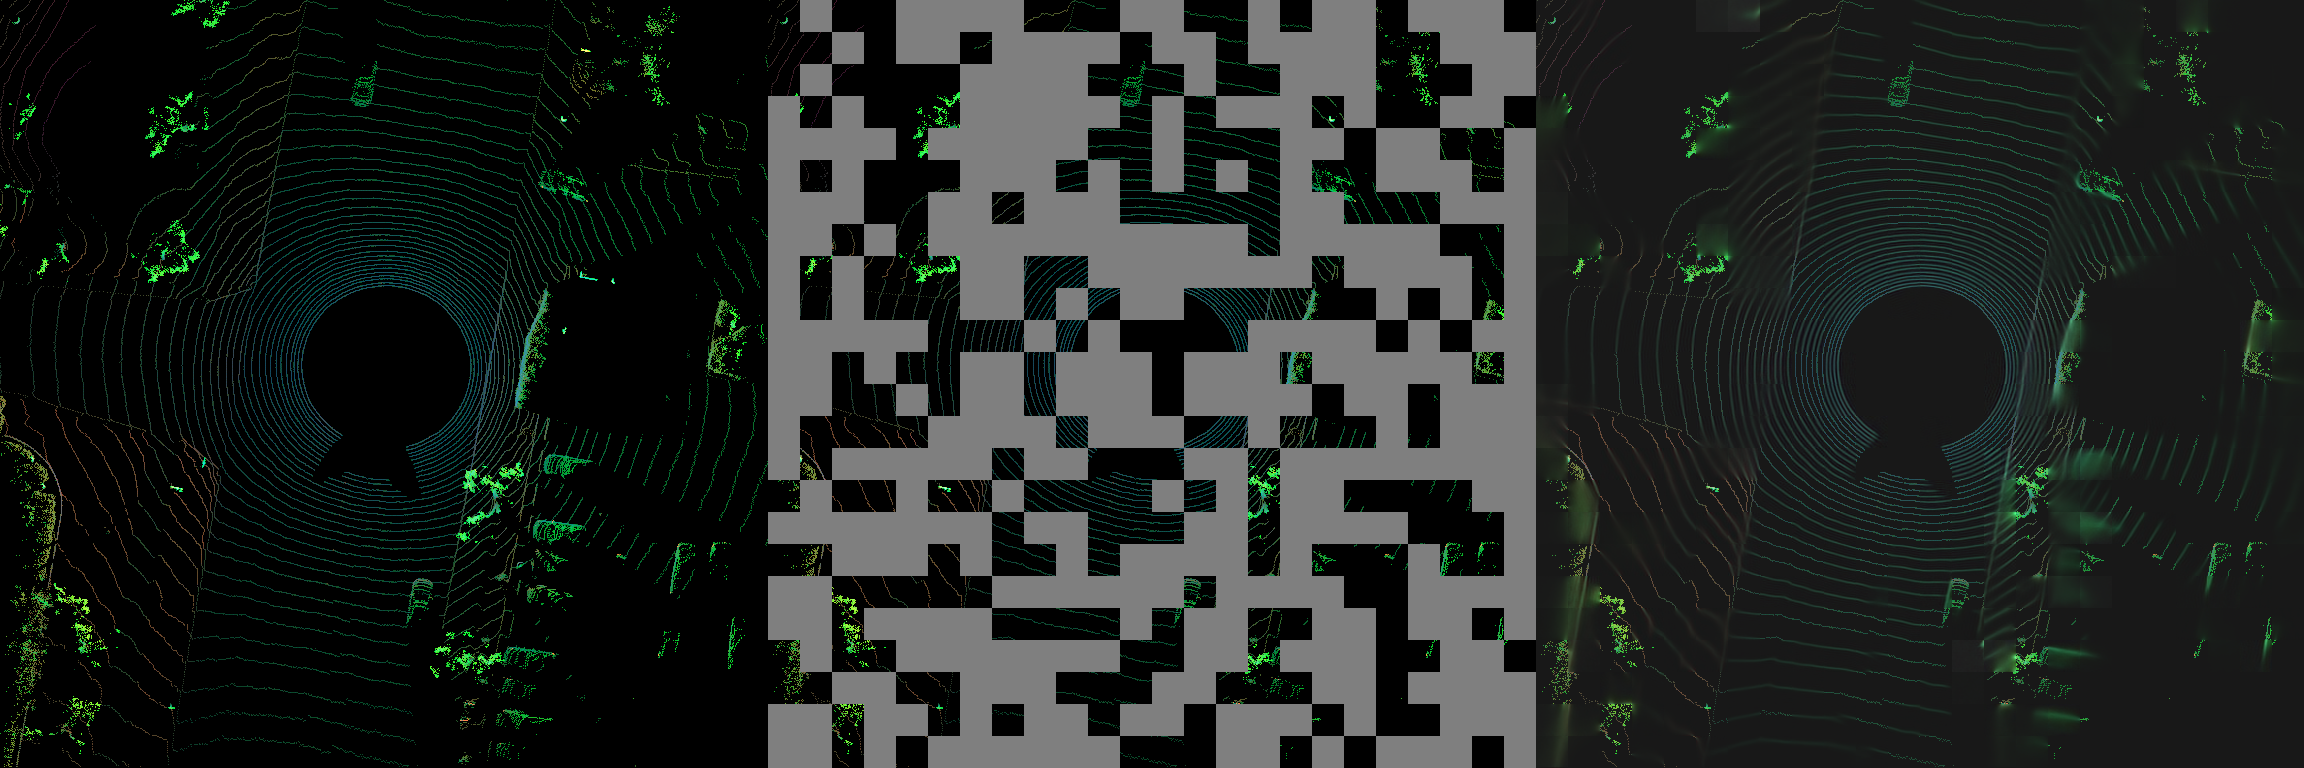
\includegraphics[width=330pt, angle=270]{pic/Hiera-Waymo.png}
        \mainfont\fontsize{9pt}{9pt}\selectfont\caption{ \mainfont\fontsize{9pt}{9pt}\selectfont Masked Autoencoding 
        (MAE) of Bird's Eye View Point Cloud Representation on Waymo Open Perception Dataset. From top to bottom: Input, Masked, Reconstruction}
        \label{fig:mae_img}
        \end{wrapfigure}
    
    During my Bachelor's degree at the Karlsruhe Institute of Technology (KIT), I focused my studies in computational mechanics. This enabled me to develop a comprehensive understanding of tensor algebra, tensor analysis and optimisation. In my Bachelor's thesis, supervised by Prof. Thomas Böhlke, I conducted research into algorithms for generating higher-order irreducible tensor representations in the context of mechanical texture development. I explored the field of computer vision and machine learning through the exceptional course on machine vision taught by Dr Martin Lauer. It was immediately apparent that the mathematical methods employed in continuum mechanics were highly transferable, which inspired me to pursue a career in this field.

    Motivated by the course on Machine Vision I applied for the internship at SICK AG, where I contributed to the embedded application layer of a smart 3D-ToF camera. The camera is used to detect obstacles on mobile agents within indoor environments using classical ML methods. In discussions with colleagues, it was determined that the lack of labelled point cloud data were the main reason for the slow implementation of deep learning, further emphazising the importance of self-supervised and unsupervised learning techniques. During my internship and period as a working student, I developed my skills as a software engineer and became a more effective team player through hands-on experience and collaboration.

    As part of my Information Technology major field, I had the opportunity to participate in the Data Driven Engineering I/II course series by Dr. Cihan Ates, where I built a strong foundation in machine learning. In the context of my research project, entitled "Energy Consumption Prediction at High Granularity", I competed at the lecture accompanying project contest, where I was placed in the top three. I gained valuable experience in the practical application of  both classical regression and forecasting methods and recurrent neural network approaches. In the second Data Driven Engineering course, my team and I worked on particle velocity and uncertainty estimation using convolutional autoencoders based on a variance attenuation loss. 



\begin{minipage}[t]{504pt}
\begin{minipage}[t]{350pt}
\setlength{\parindent}{\myindent}
\setlength{\parskip}{\myparskip}

 \vspace*{-8pt}


 \section{Past research}
 - Object Detection

 - Self Supervised Learning

 - Multi-Modal Fusion
 
 - Frame failure as big learning no paper
 
\vspace*{-6pt}

\end{minipage}
\hspace{13pt}\begin{minipage}[t]{140pt}
\begin{figure}[H]
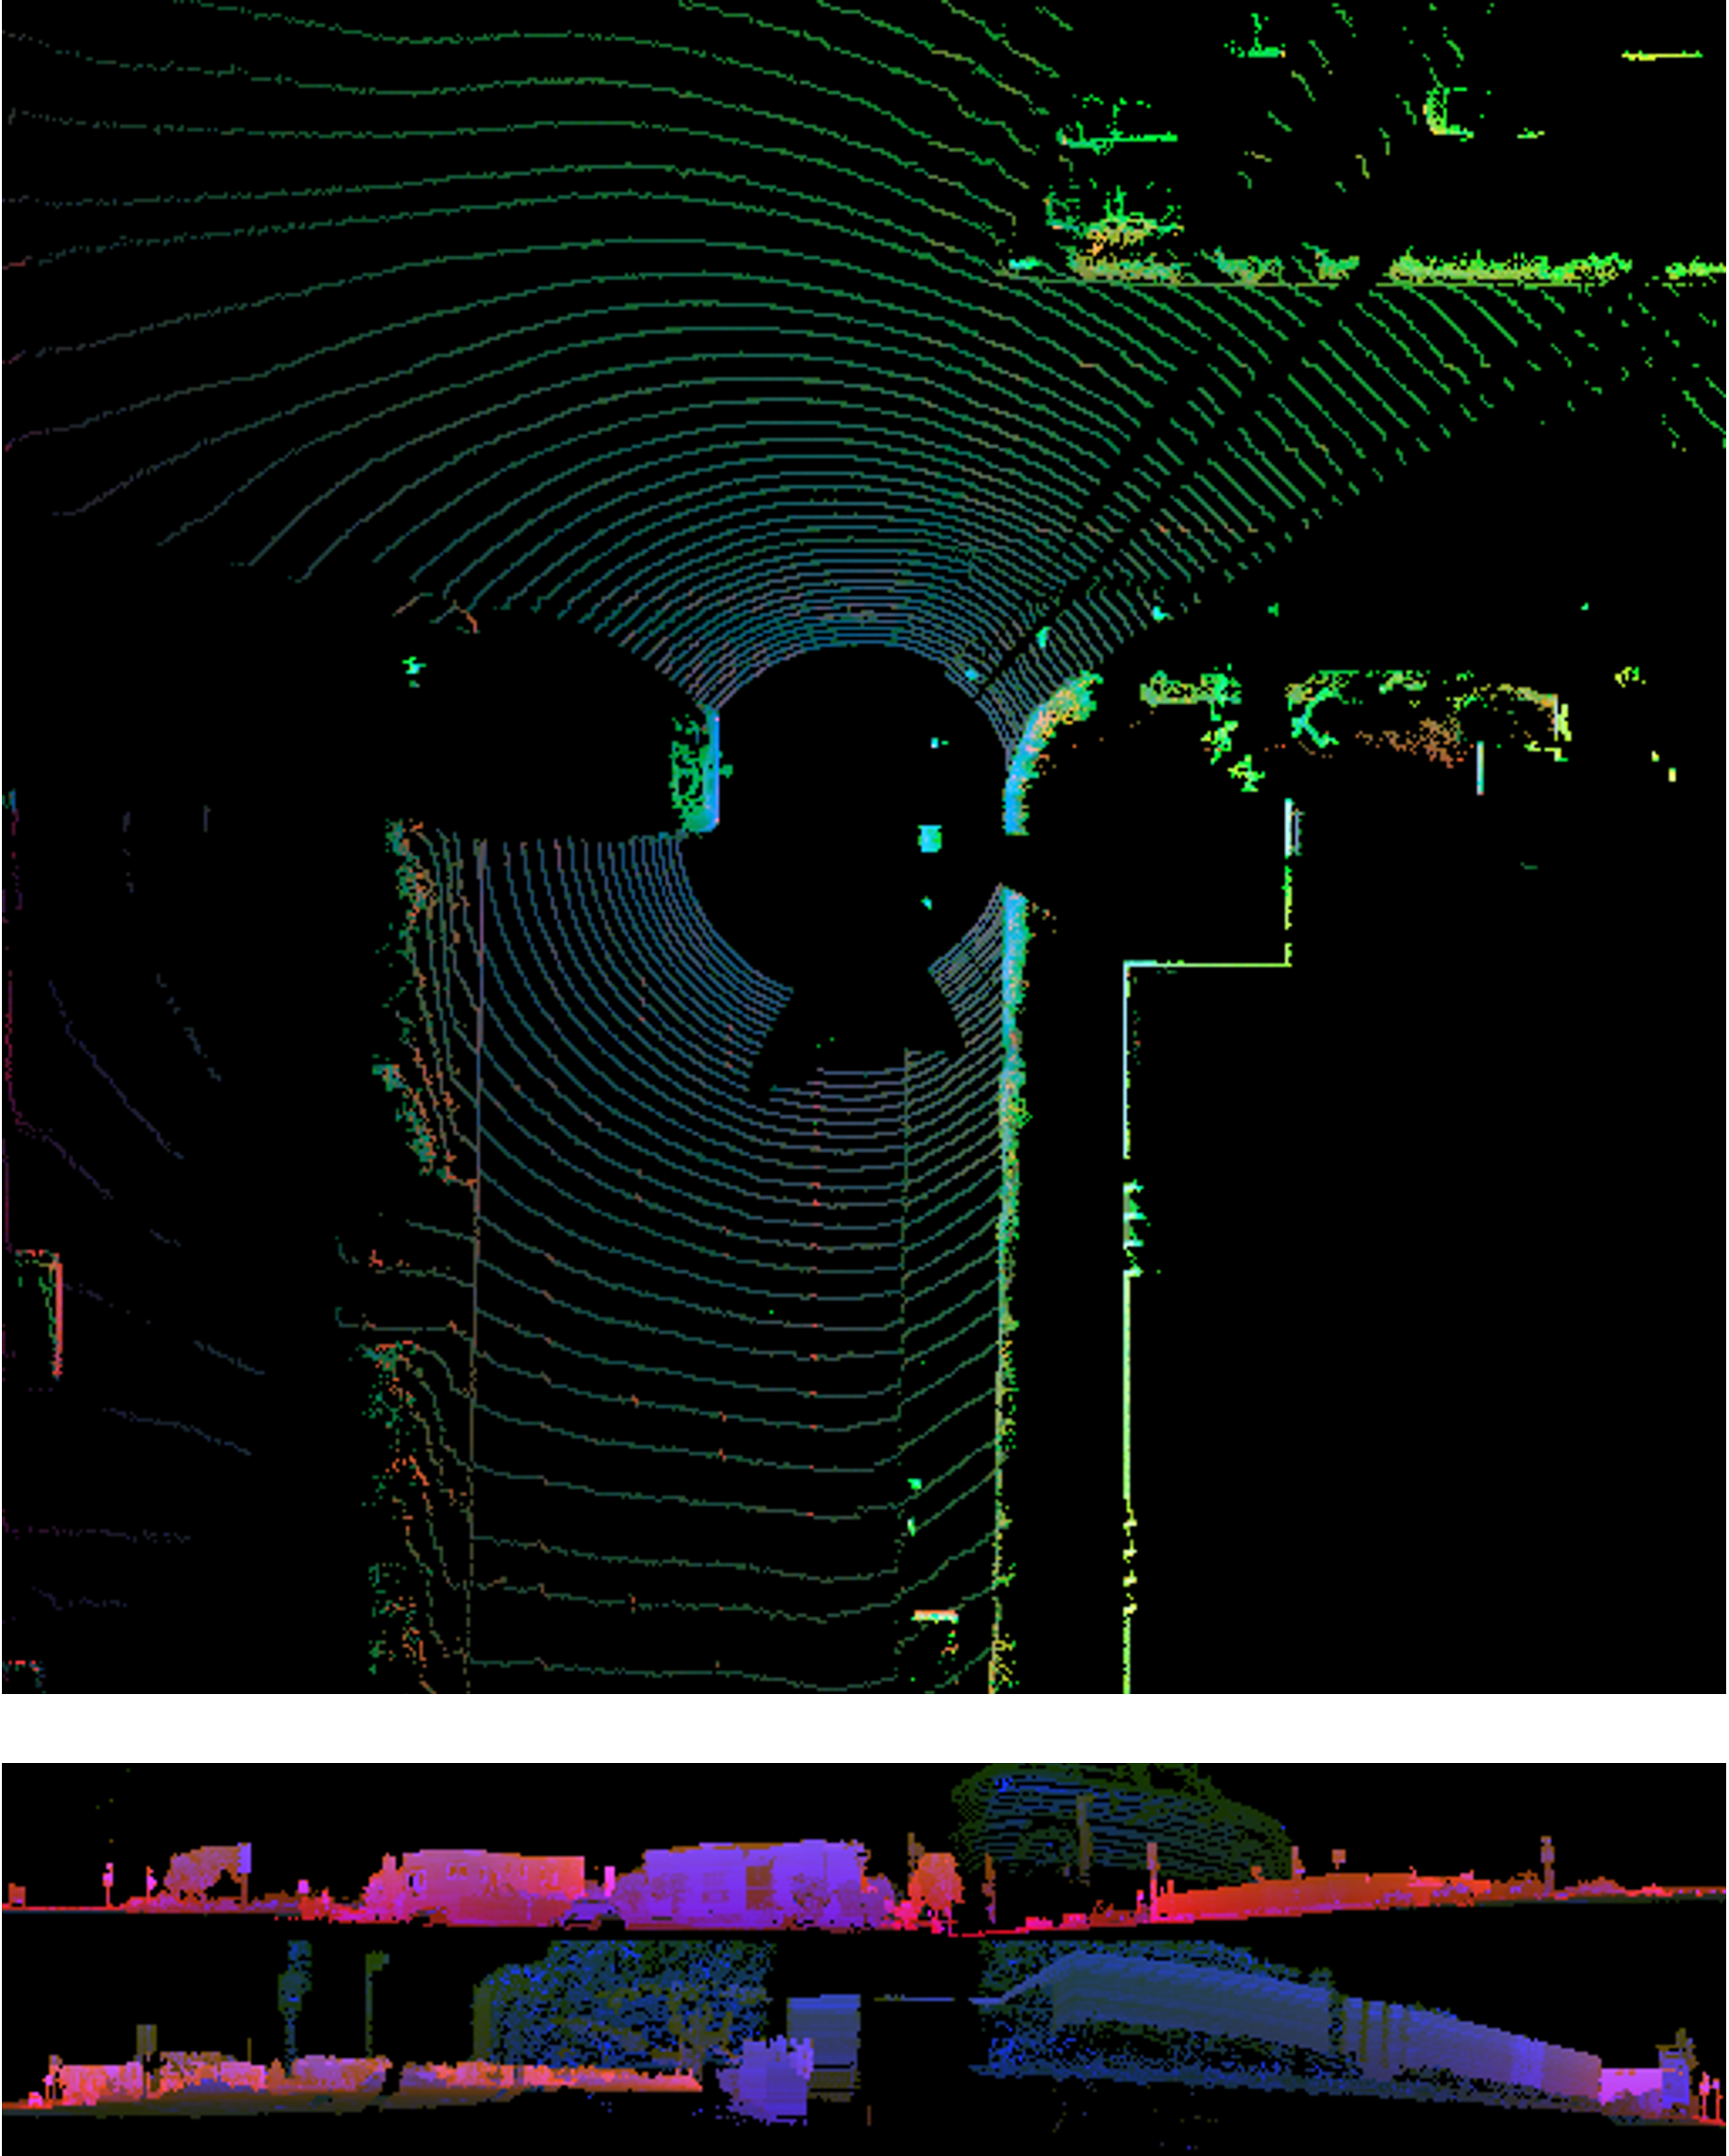
\includegraphics[width=140pt]{pic/fusion.png}
\end{figure}
\end{minipage}
\end{minipage}


\section{Future research agenda}
- Coming from perception

- Currently following the line of research of nerf pixel nerf, gaussian splatting and mvsplat (technical, perception)

- Self supervised representation learning and pretraining (conceptual)

- Curriculum learning in combination with regularizing the learning process (conceptual))
\section{Student mentoring}
- Thesis students
\subsection{\textbf{ELLIS PhD Program and Advisor}}
I am eager to delve into independent research while collaborating with fellow researchers to exchange ideas and insights. I look forward to mentoring students and assisting them with their research projects. The opportunity to conduct intensive research at the lab of my future ELLIS advisor is exciting. 

In particular I am interested in working with Prof. Dr. Abhinav Valada and Prof. Dr.-Ing. Andreas Geiger as my research interests strongly align with their work on perception and scene understanding.

The opportunity to collaborate with top-tier laboratories across Europe under the mentorship of renowned researchers in machine learning and its applications such as computer vision is unique withing the ELLIS Program. Its environment is ideal for pursuing novel fundamental and interdisciplinary research. With my solid research background, my software engineering expertise, and well aligned interests with the program’s faculty, I am confident that I am a suited fit to contribute and excel within the ELLIS PhD program.
% **** **** **** **** **** 

% font size for the references
\mainfont\fontsize{6pt}{6pt}\selectfont

\bibliographystyle{unsrt}
\bibliography{ref.bib}	

\end{document}
